\documentclass[10pt,a4paper]{article}

% Encoding and Fonts
\usepackage[utf8]{inputenc}
\usepackage[T1]{fontenc}
\usepackage{ebgaramond}
% Add this to your preamble if not already present
\usepackage{tikz}
\usetikzlibrary{arrows.meta, positioning, shapes.multipart, calc}
\usepackage{float} % For the [H] placement specifier
% Math and Symbols
\usepackage{amsmath, amsfonts, amssymb}
\usepackage{bm}

% Graphics and Figures
\usepackage{graphicx}
\usepackage{pgfgantt}
\usepackage{tikz}

% Hyperlinks
\usepackage{hyperref}
\hypersetup{
    colorlinks=true,
    linkcolor=blue,
    urlcolor=blue,
    citecolor=blue
}

% Page Layout
\usepackage{geometry}
\geometry{a4paper, margin=0.9in}

% Header and Footer
\usepackage{fancyhdr}
\pagestyle{fancy}
\fancyhf{}
\setlength{\headheight}{15pt}
\fancyhead[L]{\small Hybrid Data Augmentation and Explainable AI for ICD Code Prediction}
\fancyhead[R]{\small MTech Project Proposal}
\fancyfoot[C]{\thepage}

% Section Formatting
\usepackage{titlesec}
\titleformat{\section}
  {\normalfont\Large\bfseries\color{blue}}{\thesection}{1em}{}[{\titlerule[0.8pt]}]

% Paragraph Formatting
\usepackage{parskip}
\setlength{\parindent}{0pt}

% Lists
\usepackage{enumitem}
\setlist[itemize]{leftmargin=*, label=--}

% Colors
\usepackage{color}

% Captions
\usepackage{caption}

% Tables
\usepackage{array}
\usepackage{booktabs}

% Improved Typography
\usepackage{microtype}

% Bibliography
\usepackage{cite}

% Gantt Chart Styling
\usepackage{pgfgantt}
\usepackage{pgfplots}

% Document Information
\title{Hybrid Data Augmentation and Explainable AI for ICD Code Prediction}
\author{
    Kaustabh Ganguly \\
    Roll Number: CH23M514 \\
    Mentors: Samyabrata Chakraborty, Debopam Nanda \\
}
\date{September 22, 2024}

\begin{document}

\maketitle

% 1. Project Title
\section{Project Title}
\textbf{Hybrid Data Augmentation and Explainable AI for ICD Code Prediction}

\section{Project Particulars}
\textbf{Area and Sub-Areas}: 
\begin{itemize}
    \item \textbf{Medical Natural Language Processing (NLP)}: Advanced processing of clinical narratives for information extraction and understanding.
    \item \textbf{Transformer-Based Deep Learning Models}: Utilizing state-of-the-art architectures for complex predictive modeling tasks in healthcare.
    \item \textbf{Hybrid Data Augmentation Techniques}: Combining Retrieval Augmented Generation and ontology-based methods to address data scarcity, especially for rare ICD codes.
    \item \textbf{Knowledge Representation and Integration}: Leveraging medical ontologies and knowledge graphs to enrich data and model comprehension.
    \item \textbf{Explainable Artificial Intelligence (XAI)}: Implementing interpretability techniques to ensure transparency and trustworthiness of the model.
    \item \textbf{Clinical Decision Support Systems}: Enhancing healthcare delivery by integrating AI-driven insights into clinical workflows.
    \item \textbf{Multi-Label Multi-Class Classification}: Addressing the challenges of predicting multiple ICD codes from clinical text.
    \item \textbf{Human-in-the-Loop Machine Learning}: Incorporating clinician feedback to refine model predictions and ensure clinical relevance.
\end{itemize}

\textbf{Duration}: 11 months (September 2024 - July 2025), including a 2-month buffer

% 3. Student and Mentor Particulars
\section{Student and Mentor Particulars}
\textbf{Student}: Kaustabh Ganguly (CH23M514)

\textbf{Mentors}: 
\begin{itemize}
    \item Samyabrata Chakraborty (AI/Domain Expert)
    \item Debopam Nanda (AI Expert)
\end{itemize}

\section{Project Summary}
The manual annotation of \textbf{International Classification of Diseases (ICD) codes} from clinical text is labor-intensive and error-prone, impacting healthcare efficiency, billing accuracy, and medical research. My project aims to accurately predict ICD codes from clinical narratives, with a focus on \textbf{rare medical codes} often overlooked due to data scarcity.

Driven by the critical need to improve healthcare outcomes, I propose a comprehensive approach that transforms raw clinical text into structured representations by extracting medical entities and mapping them to ontologies like \textbf{SNOMED CT} and \textbf{RxNorm}. I will then convert this enriched data into embeddings using \textbf{transformer-based models}.

To enhance the model's ability to predict rare ICD codes, I will implement a \textbf{hybrid data augmentation strategy} that combines \textbf{Retrieval Augmented Generation (RAG)} with \textbf{ontology-based techniques}. RAG will retrieve detailed descriptions and related information for each ICD code from external sources such as \textbf{PubMed}, \textbf{Wikipedia}, and the \textbf{WHO API}, expanding the code descriptions to include comprehensive information like symptoms, diagnoses, and treatments. These enriched descriptions will form a semantic space that aligns with the embeddings of clinical text.

The model will map clinical text embeddings to this expanded description space, effectively predicting ICD codes by matching clinical narratives to detailed code representations. This approach leverages the complex interplay between symptoms, diagnoses, procedures, and medications, captured through \textbf{knowledge graphs} constructed from medical ontologies.

Additionally, I will generate \textbf{synthetic clinical notes} for each ICD code, particularly the rare ones, using generative models such as \textbf{GANs}. These synthetic notes will incorporate entities from \textbf{RxNorm}, \textbf{SNOMED CT}, and other ontologies, ensuring medical accuracy and coherence.

To handle the multi-label, multi-class classification challenge, I will implement advanced techniques like \textbf{label embedding}, \textbf{hierarchical classification}, and \textbf{label grouping}. These strategies will capture relationships between ICD codes and improve the model's performance and efficiency.

By integrating these methodologies, the model will predict a set of relevant ICD codes from clinical text, even for codes not present in the training dataset, thus improving coverage and accuracy. The use of \textbf{explainability techniques} such as \textbf{SHAP}, \textbf{LIME}, and \textbf{Integrated Gradients} will provide interpretable insights into predictions, enhancing clinician trust and facilitating acceptance.

The deliverables include an \textbf{open-source toolkit} that automates the ICD coding process, reduces administrative burdens, and contributes to improved healthcare outcomes by enhancing accuracy and reliability in clinical settings.

\section{Objectives}
\begin{enumerate}
    \item \textbf{Develop a transformer-based model} that maps clinical text embeddings to enriched ICD code embeddings, integrating unstructured clinical narratives with structured medical knowledge for accurate multi-label ICD code prediction.
    \item \textbf{Implement a hybrid data augmentation strategy} combining Retrieval Augmented Generation (RAG) with ontology-based methods to generate synthetic clinical notes and expand ICD code descriptions, focusing on rare ICD codes.
    \item \textbf{Leverage knowledge graphs and ontologies} (SNOMED CT, RxNorm, ICD-10-CM) to ensure medical coherence in data augmentation and enhance the model's understanding of medical concepts and relationships.
    \item \textbf{Employ advanced classification techniques} such as label embedding, hierarchical classification, and label grouping to effectively manage the large label space and improve prediction of rare ICD codes.
    \item \textbf{Integrate explainability techniques} like SHAP, LIME, and Integrated Gradients to provide transparent insights into model predictions, facilitating clinician acceptance.
    \item \textbf{Achieve a significant improvement in evaluation metrics}, aiming for at least a 10\% increase in macro F2-score on rare ICD codes over baseline models.
    \item \textbf{Develop an open-source toolkit} that automates the ICD coding process, providing a valuable resource for the research community and healthcare industry.
\end{enumerate}

% 6. Current State of the Art
\section{Current State of the Art}
Accurate prediction of \textbf{ICD codes} from clinical text is crucial for efficient healthcare operations. Transformer-based models like BERT, BioBERT, ClinicalBERT, and Longformer have significantly improved automatic ICD coding by capturing contextual nuances in medical narratives \cite{si2019enhancing, sheu2022survey}. However, predicting \textbf{rare ICD codes} remains challenging due to data imbalance and scarcity.

To address this, researchers have explored \textbf{data augmentation techniques}. Wang et al. \cite{wang2019clinical} utilized GANs to generate synthetic clinical notes, enhancing model performance on rare codes. \textbf{Retrieval Augmented Generation (RAG)} combines retrieval mechanisms with generative models to produce contextually relevant synthetic data, offering a promising solution.

Integrating \textbf{knowledge graphs} from ontologies like \textbf{SNOMED CT} and \textbf{RxNorm} enriches models with structured medical knowledge \cite{gong2023explainable}. This integration helps models understand complex relationships between medical entities, improving prediction accuracy.

\textbf{Explainable AI (XAI)} is essential for clinical applications to gain trust from healthcare professionals. Techniques like \textbf{SHAP}, \textbf{LIME}, and \textbf{Integrated Gradients} have been successfully applied to transformer-based models in multi-label classification contexts, providing interpretable insights even with complex architectures \cite{fantozzi2024explainability, volkov2024local, szczepanski2021new, gucukbel2023evaluating}. \textbf{Human-in-the-loop} approaches allow clinician feedback to refine models, aligning them with real-world clinical practice \cite{panda2023clinician}.

Despite these advancements, gaps persist in effectively combining these techniques to improve prediction of rare ICD codes while ensuring model interpretability. Specifically, there is limited research on integrating RAG with knowledge graphs and seamless incorporation of XAI methods within such frameworks. Additionally, tools like \textbf{cTAKES}, \textbf{MedSpaCy}, and \textbf{MedCat} play a crucial role in entity recognition and linking, but their integration within hybrid augmentation and explainable frameworks remains underexplored. My project aims to bridge these gaps by integrating RAG-based data augmentation, knowledge graphs, and explainability methods into a unified framework.

% 7. Work Plan
\section{Work Plan}
The project will be executed over 11 months (September 2024 - July 2025), divided into five key phases with adjusted timelines to accommodate potential challenges and ensure thorough execution:

% Gantt Chart
\begin{figure}[h]
    \centering
    \begin{ganttchart}[
        hgrid,
        vgrid,
        x unit=0.7cm,
        y unit title=0.6cm,
        y unit chart=0.6cm,
        title height=1,
        bar/.style={fill=blue!50},
        bar height=0.5
    ]{1}{11}
        \gantttitle{Project Timeline (Months)}{11} \\
        \gantttitlelist{1,...,11}{1} \\
        \ganttbar{Phase 1: Data Preparation}{1}{3} \\
        \ganttbar{Phase 2: Model Development and Evaluation}{4}{7} \\
        \ganttbar{Phase 3: Explainability Integration}{7}{9} \\
        \ganttbar{Phase 4: Deployment \& Dissemination}{8}{9} \\
        \ganttbar{Phase 5: Human-in-the-Loop System}{10}{11} \\
    \end{ganttchart}
    \caption{Gantt Chart of Project Phases}
\end{figure}

\textbf{Detailed Phases and Tasks}:

The project spans five key phases over 11 months:

\begin{itemize}
    \item \textbf{Phase 1: Data Preparation (Months 1-3)} involves data acquisition, preprocessing, entity extraction, and ontology mapping using tools like cTAKES, MedSpaCy, and MedCat, along with knowledge graph construction.
    \item \textbf{Phase 2: Model Development and Evaluation (Months 4-7)} includes hybrid data augmentation using RAG and ontology-based methods to generate synthetic clinical notes and expand ICD code descriptions, model architecture design with transformer-based embeddings, knowledge integration, handling multi-label classification through label embedding and hierarchical classification, model training and validation using cross-validation, performance evaluation with standardized metrics (Precision, Recall, F1-score, F2-score), and error analysis for optimization.
    \item \textbf{Phase 3: Explainability Integration (Months 7-9)} involves integrating explainability tools like SHAP, LIME, and Integrated Gradients, and developing visualizations to present explanations to clinicians.
    \item \textbf{Phase 4: Deployment \& Dissemination (Months 8-9)} focuses on toolkit development, documentation, and final reporting.
    \item \textbf{Phase 5: Human-in-the-Loop System (Months 10-11)} entails creating an interface for clinicians to review predictions and outlining a framework for incorporating clinician feedback.
\end{itemize}

\section{Architecture Diagram}
\begin{figure}[H]
    \centering
    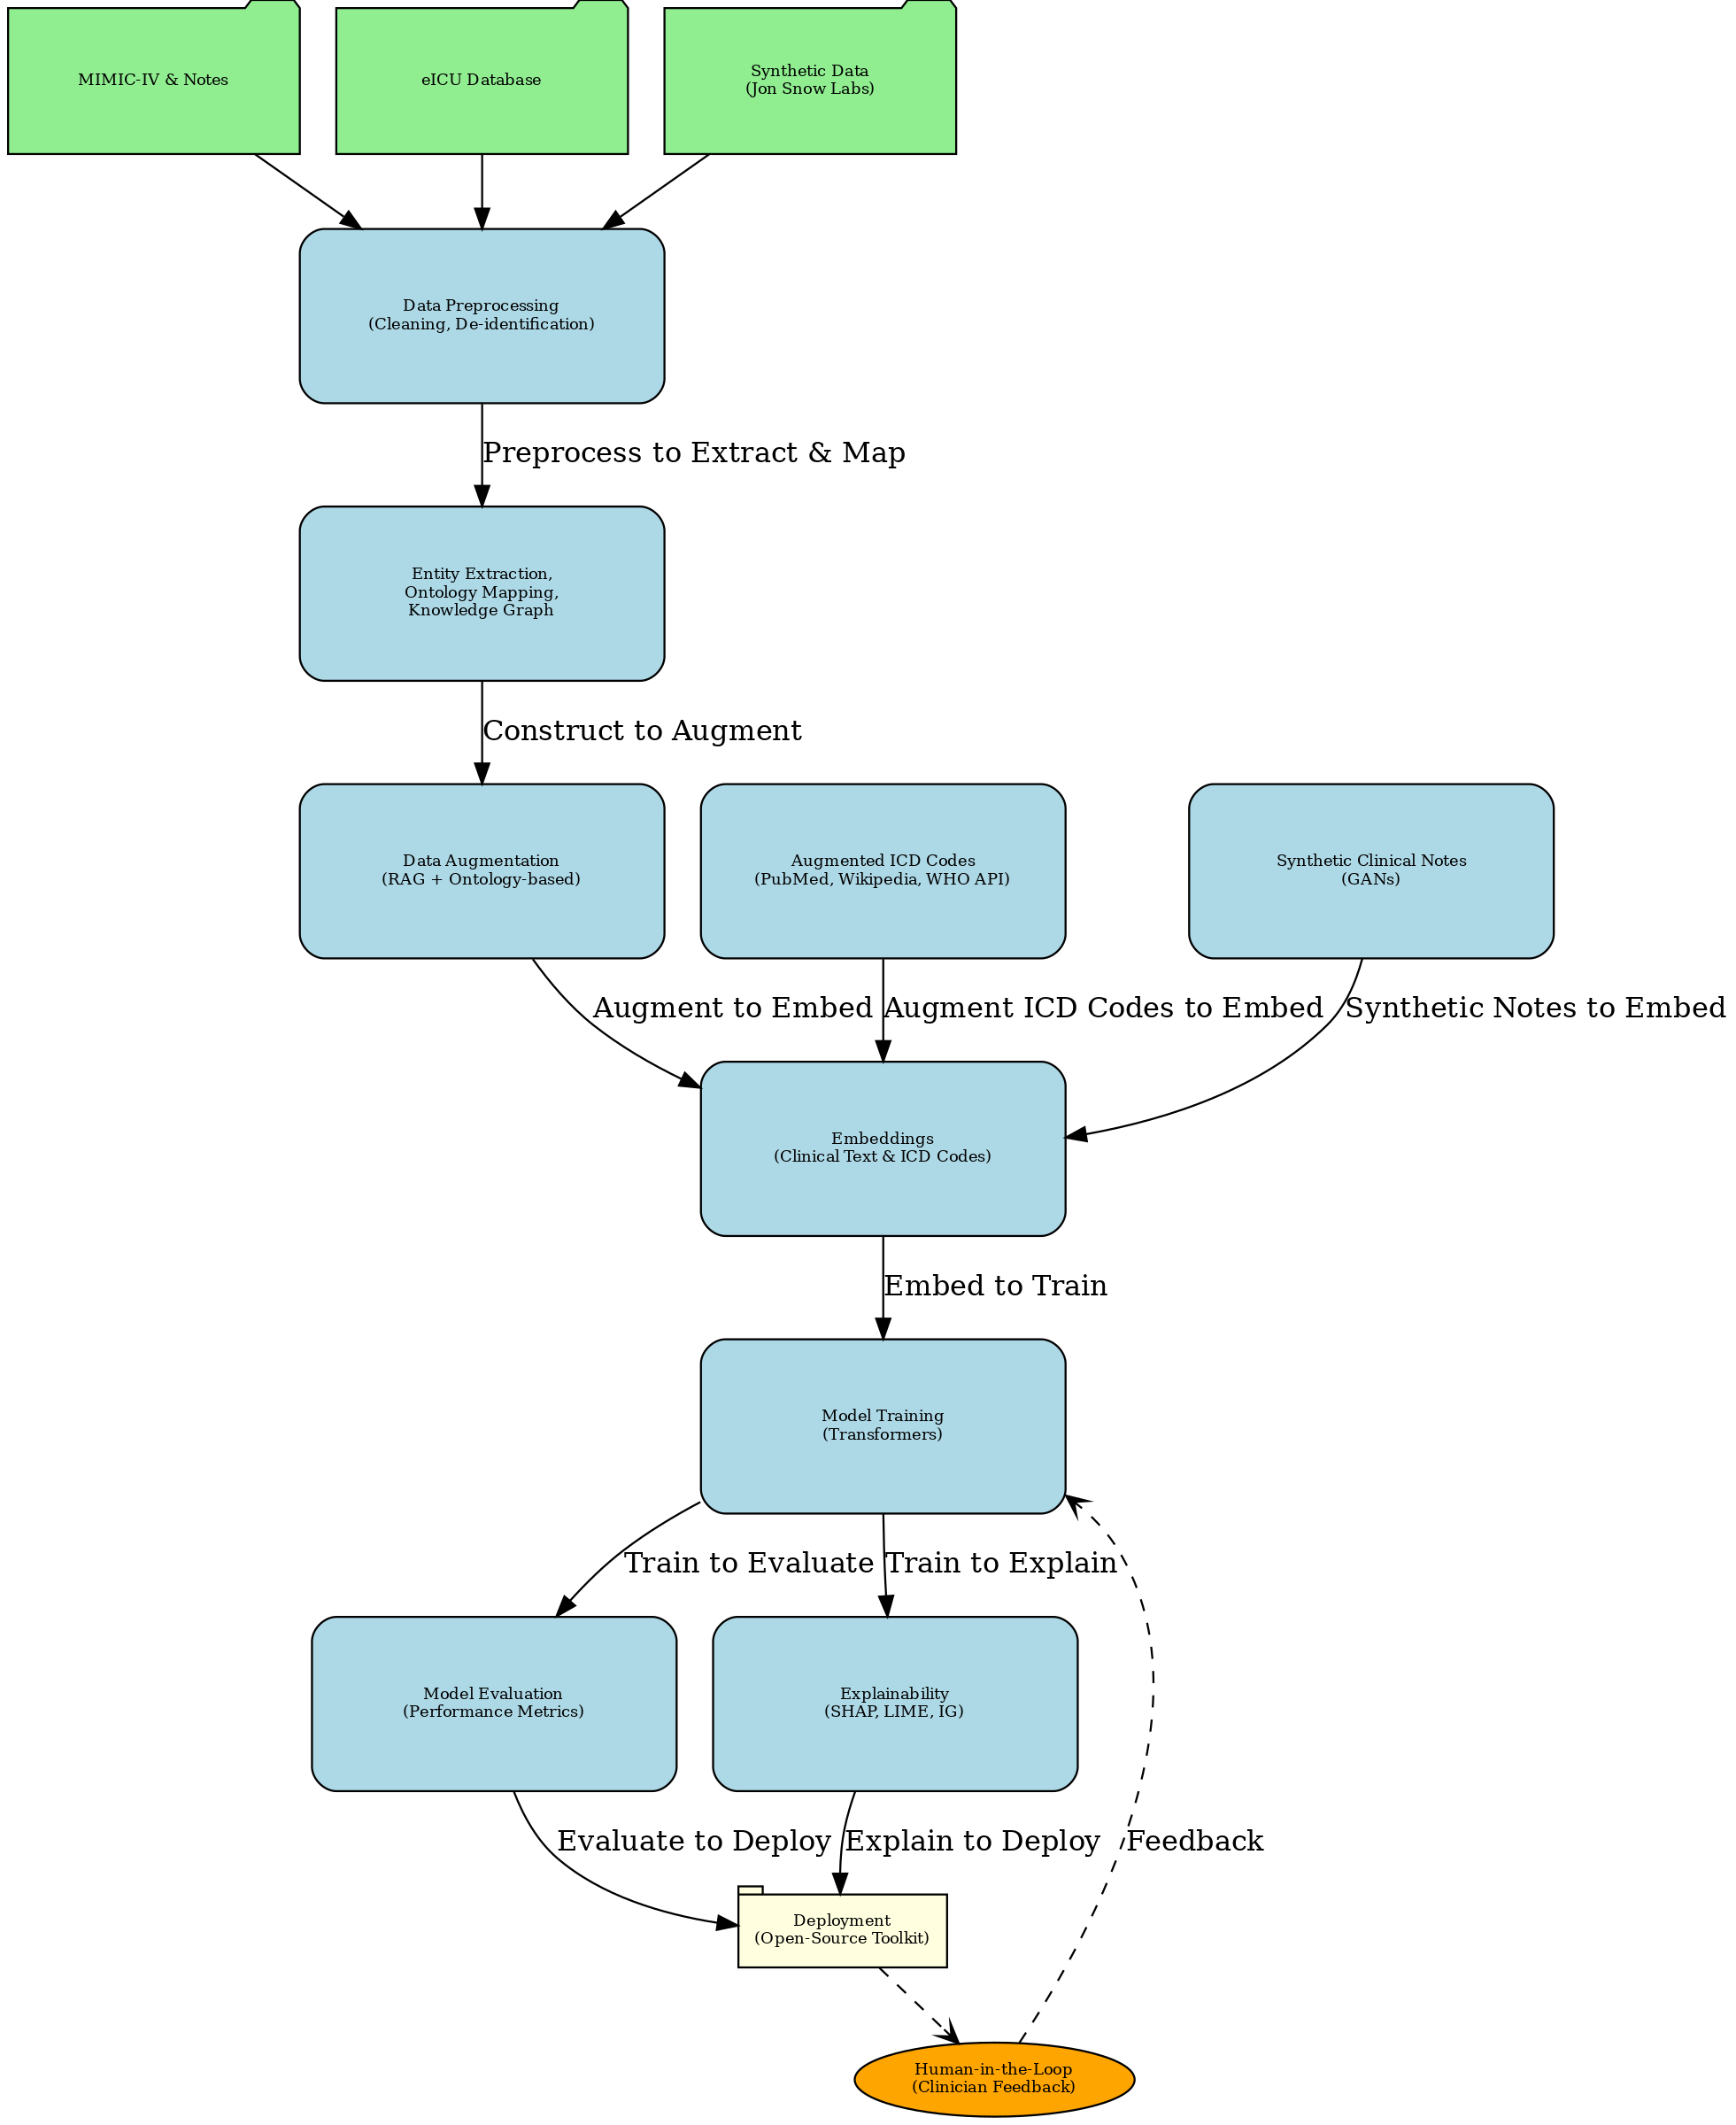
\includegraphics[width=\textwidth]{architecture_diagram_top_down.png}
    \caption{Architecture Diagram of the Project}
\end{figure}

% 9. Data Sets
\section{Data Sets}
The project utilizes multiple datasets to ensure comprehensive coverage and robustness:

\textbf{Primary Datasets:}
\begin{itemize}
    \item \textbf{MIMIC-IV Clinical Database}: Over 40,000 patient records with unstructured clinical notes linked to ICD codes.
    \item \textbf{MIMIC-IV Notes}: Detailed clinical notes extracted from the MIMIC-IV database.
    \item \textbf{eICU Collaborative Research Database}: Data from intensive care units, providing critical patient information.
    \item \textbf{Jon Snow Labs Synthetic Data}: Synthetic clinical data for augmenting training datasets.
\end{itemize}

\textbf{Additional Resources:}
\begin{itemize}
    \item \textbf{WHO API}: To fetch up-to-date ICD-10-CM codes and related medical information.
    \item \textbf{NBME}: Medical education resources for supplementary clinical scenarios.
    \item \textbf{External Medical Literature}: Incorporating information from PubMed and detailed ICD code descriptions to enrich data augmentation.
\end{itemize}

All data handling will comply with ethical guidelines and data use agreements, ensuring patient privacy and data security.

% 10. Methodology
\section{Methodology}

To tackle the multi-label, multi-class classification challenge with over 73,000 ICD codes, the methodology involves several key components:

\textbf{Data Representation}:
\begin{itemize}
    \item \textbf{Entity Extraction and Ontology Mapping}: Convert raw clinical text into structured data by extracting medical entities and mapping them to \textbf{SNOMED CT} and \textbf{RxNorm}.
    \item \textbf{Augmented ICD Code Descriptions}: Expand ICD-10-CM code descriptions using \textbf{Retrieval Augmented Generation (RAG)} to include detailed information from \textbf{PubMed}, \textbf{Wikipedia}, and \textbf{WHO API}.
    \item \textbf{Embedding Spaces}: Create embeddings for both clinical text and ICD code descriptions using transformer-based models, allowing for semantic alignment.
    \item \textbf{Label Representation}: Use label embeddings to capture relationships between ICD codes, facilitating multi-label predictions.
\end{itemize}

\textbf{Model Architecture}:
\begin{itemize}
    \item \textbf{Transformer-Based Models}: Utilize models like \textbf{ClinicalBERT} or \textbf{Longformer} to encode clinical text and code descriptions.
    \item \textbf{Knowledge Integration}: Incorporate knowledge graph embeddings to enrich model understanding of medical concepts.
    \item \textbf{Mapping Mechanism}: Implement a mechanism to map clinical text embeddings to ICD code embeddings.
    \item \textbf{Multi-Label Classification Techniques}: Employ \textbf{label embedding}, \textbf{hierarchical classification}, and \textbf{label grouping} to handle the extensive label space.
\end{itemize}

\textbf{Data Augmentation}:
\begin{itemize}
    \item \textbf{Synthetic Clinical Note Generation}: Use generative models to create synthetic clinical notes for rare ICD codes, incorporating ontology-based entities.
    \item \textbf{Hybrid Augmentation Strategy}: Combine RAG with ontology-based methods to enrich the training dataset.
\end{itemize}

\textbf{Handling Class Imbalance}:
\begin{itemize}
    \item \textbf{Loss Functions}: Employ \textbf{focal loss} to focus on hard-to-classify and rare codes.
    \item \textbf{Sampling Techniques}: Use oversampling of rare classes or undersampling of common classes.
\end{itemize}

\textbf{Prediction and Thresholding}:
\begin{itemize}
    \item \textbf{Probability Outputs}: Configure the model to output probabilities for each ICD code using a Sigmoid activation function.
    \item \textbf{Threshold Optimization}: Apply probability thresholds or select top-N codes based on confidence scores.
\end{itemize}

\textbf{Evaluation Metrics}:

To comprehensively evaluate the performance of the multi-label, multi-class ICD code prediction model, I will employ a set of standardized evaluation metrics:

\begin{itemize}
    \item \textbf{Precision, Recall, and F1-score}: Calculated on a per-class basis and aggregated using micro and macro averaging to provide insights into both overall performance and performance on individual ICD codes.
    \item \textbf{F2-score}: Defined as:

    \[
    F_{2} = (1 + 2^2) \times \frac{\text{Precision} \times \text{Recall}}{(2^2 \times \text{Precision}) + \text{Recall}}
    \]

    The F2-score places more emphasis on recall than precision, which is crucial in the medical domain where failing to identify a relevant ICD code (false negative) can have more severe consequences than incorrectly assigning an extra code (false positive). This aligns with the goal of ensuring that all pertinent medical conditions are captured.
    \item \textbf{Area Under the ROC Curve (AUC-ROC)}: Measures the model's ability to distinguish between classes across all thresholds, providing a global perspective on performance.
    \item \textbf{Area Under the Precision-Recall Curve (AUC-PR)}: Particularly valuable for imbalanced datasets, as it focuses on the performance related to the positive class, which is essential for rare ICD codes.
    \item \textbf{Hamming Loss}: Calculates the fraction of incorrect labels to the total number of labels, offering insight into the overall error rate of the model.
    \item \textbf{Subset Accuracy}: The strictest metric, which considers a prediction correct only if all predicted ICD codes exactly match the true set, providing a holistic measure of performance.
\end{itemize}

\textbf{Explainability Integration}:
\begin{itemize}
    \item \textbf{Explainability Techniques}: Integrate \textbf{SHAP}, \textbf{LIME}, and \textbf{Integrated Gradients} to interpret model predictions.
    \item \textbf{Interpretability}: Enhance transparency by explaining how the model maps clinical text to ICD codes.
\end{itemize}

By standardizing these metrics at the outset, I will ensure consistent evaluation throughout the model development journey.

% 11. Expected Deliverables/Outcomes
\section{Expected Deliverables/Outcomes}
\begin{enumerate}
    \item \textbf{An advanced, explainable model} for ICD code prediction, achieving significant improvements in evaluation metrics (e.g., at least a 10\% increase in macro F2-score on rare ICD codes over baseline models).
    \item \textbf{A comprehensive set of enriched ICD code embeddings} derived from expanded code descriptions and knowledge graphs.
    \item \textbf{An open-source toolkit} including data processing pipelines, model code, and synthetic data generation methods.
    \item \textbf{Detailed experimental records} documenting model configurations and performance metrics.
    \item \textbf{Enhanced model interpretability} through integrated explainability features, enabling clinicians to understand and trust predictions.
    \item \textbf{A framework for human-in-the-loop integration}, outlining how clinician feedback can refine the model.
\end{enumerate}

% 12. Significance of the Expected Outcomes
\section{Significance of the Expected Outcomes}
This project will:
\begin{itemize}
    \item \textbf{Advance medical NLP} by integrating unstructured and structured data for improved ICD code prediction.
    \item \textbf{Improve clinical workflows} by automating and enhancing the accuracy of the ICD coding process.
    \item \textbf{Enhance patient care and research} through comprehensive and precise medical coding.
    \item \textbf{Promote transparency and trust} in AI systems via explainable models.
    \item \textbf{Provide a valuable resource} to the research community through an open-source toolkit and documented methodologies.
\end{itemize}

\section{Implementation Arrangements}
I will conduct the project under the guidance of mentors Samyabrata Chakraborty and Debopam Nanda, collaborating actively with clinicians who will provide essential domain expertise and feedback. Regular bi-weekly meetings with healthcare professionals will ensure that the model aligns with clinical needs, allowing for the incorporation of their insights into the development process. Additionally, I will adopt an agile methodology, organizing the project into two-week sprints with specific goals and deliverables, followed by progress reviews and necessary adjustments based on ongoing feedback.

\section{Resource Requirements} 
The project will utilize \textbf{Google Colab Pro} for initial experiments, \textbf{AWS/GCP credits} for scalable training, and a \textbf{local machine} with 32GB RAM, an NVIDIA RTX 3060 GPU, and 2TB storage for data processing and model training. The software tools will include open-source platforms such as \textbf{Python}, \textbf{PyTorch/TensorFlow}, \textbf{Hugging Face Transformers}, \textbf{SHAP}, and \textbf{LIME}, all freely available without the need for additional licenses. For entity linking, \textbf{cTAKES}, \textbf{MedSpaCy}, and \textbf{MedCat} will be employed for Named Entity Recognition and linking. Data access will involve secure access to the \textbf{MIMIC-IV database}, \textbf{MIMIC-IV Notes}, \textbf{eICU Collaborative Research Database}, \textbf{Jon Snow Labs synthetic data}, and medical ontologies such as \textbf{SNOMED CT}, \textbf{RxNorm}, and \textbf{ICD-10-CM} via the \textbf{WHO API}.

% 15. Risks
\section{Risks}
Potential challenges include data privacy concerns, model performance issues, integration complexity, resource limitations, and timeline delays. To mitigate these risks, I will ensure compliance with HIPAA and data use agreements through strict data anonymization and secure handling protocols. I will address model performance issues, particularly for rare codes, by employing techniques such as focal loss and per-class evaluation metrics like the F2-score to handle class imbalance. Integration complexity will be managed by modular development and thorough testing of each component. Resource limitations will be addressed by optimizing models and leveraging cloud computing resources efficiently. To prevent timeline delays, I will implement careful planning with contingency buffers and regular progress tracking to adjust plans proactively based on feedback.

\begin{thebibliography}{10}
\setlength{\itemsep}{0pt}

\bibitem{sheu2022survey}
Sheu, R.-K., et al. (2022).
\newblock A Survey on Medical Explainable AI (XAI): Recent Progress, Explainability Approach, Human Interaction and Scoring System.
\newblock \textit{Sensors}, 22(20), 8068.

\bibitem{si2019enhancing}
Si, Y., \& Roberts, K. (2019).
\newblock Enhancing Clinical Concept Extraction with Contextual Embeddings.
\newblock \textit{Journal of the American Medical Informatics Association}, 26(11), 1297–1304.

\bibitem{wang2019clinical}
Wang, S., Liu, S., \& Li, B. (2019).
\newblock Clinical Information Extraction via Deep Learning Approaches.
\newblock \textit{International Journal of Environmental Research and Public Health}, 16(14), 2565.

\bibitem{gong2023explainable}
Gong, J., et al. (2023).
\newblock Explainable Prediction of Medical Codes from Clinical Text Using Knowledge Graphs.
\newblock \textit{arXiv preprint arXiv:2303.12345}.

\bibitem{hu2023explainable}
Hu, S. Y., \& Teng, F. (2023).
\newblock An Explainable CNN Approach for Medical Codes Prediction from Clinical Text.
\newblock \textit{BMC Medical Informatics and Decision Making}, 23(1), 2.

\bibitem{panda2023clinician}
Panda, S., et al. (2023).
\newblock Towards Clinician-Preferred Segmentation: Leveraging Human-in-the-Loop for Test Time Adaptation in Medical Image Segmentation.
\newblock \textit{arXiv preprint arXiv:2301.09876}.

\bibitem{johnson2019mimic}
Johnson, A. E. W., et al. (2019).
\newblock MIMIC-IV (version 1.0).
\newblock \textit{PhysioNet}.

\bibitem{fantozzi2024explainability}
Fantozzi, P., \& Naldi, M. (2024).
\newblock The Explainability of Transformers: Current Status and Directions.
\newblock \textit{Computers}, 13(4), 92.

\bibitem{gucukbel2023evaluating}
Gucukbel, E. (2023).
\newblock Evaluating the Explanation of Black Box Decision for Text Classification.
\newblock \textit{Master's Thesis, Freie Universität Berlin}.

\bibitem{volkov2024local}
Volkov, E. N., \& Averkin, A. N. (2024).
\newblock Local Explanations for Large Language Models: A Brief Review of Methods.
\newblock In \textit{Proceedings of the IEEE International Conference on Soft Computing and Measurements}.

\bibitem{szczepanski2021new}
Szczepański, M., et al. (2021).
\newblock New Explainability Method for BERT-Based Model in Fake News Detection.
\newblock \textit{Scientific Reports}, 11(1), 23705.

\end{thebibliography}

\end{document}
